\chapter{Анализ основных причин джиттера в проводной и беспроводной сети} \label{chapt2}
Выделяют три типа джиттера \cite{clark}, которые могут быть вызваны различными причинами (рис. \ref{img:3typeJitter}):
\begin{enumerate}
  \item Выброс задержки возникает, когда один пакет в потоке оказывается задержанным на значительно больший интервал времени по отношению к другим. Это может произойти в тех случаях, когда осуществляется передача высокоприоритетного служебного трафика, когда возникают сетевые перегрузки, изменение маршрута и др. Эти случаи могут привести к проблеме неограниченного изменения оценки управляющей системы за один шаг.
  \item Постоянный джиттер - это передача пакетов с примерно постоянным изменением задержки;
  \item Скачок задержки, который может возникнуть из-за всплеска пакетной активности. Это явление, как правило, связано с перегрузками линии доступа или изменением маршрута. Скачок задержки может привести систему управления в неустойчивое состояние, что приводит к нежелательным последствиям.
\end{enumerate}

\begin{figure} [h] 
  \center
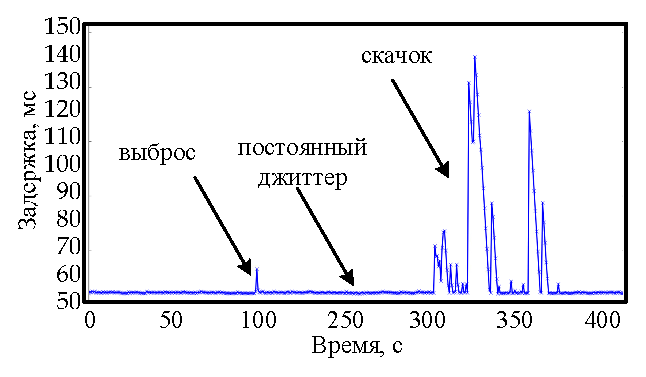
\includegraphics{3typeJitter.eps}
  %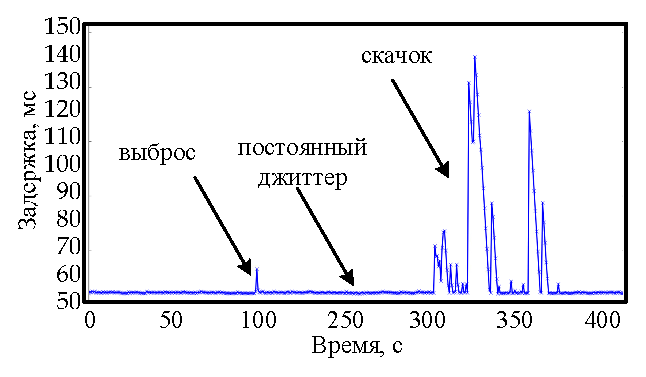
\includegraphics [scale=0.9] {3typeJitter.eps}
%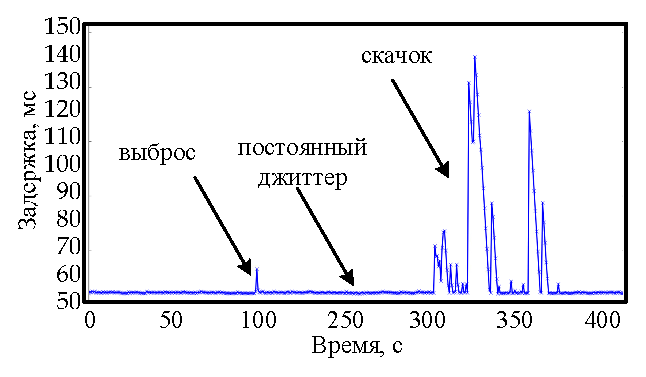
\includegraphics {3typeJitter}
  \caption{График задержек в реальной сети \cite{clark}} 
  \label{img:3typeJitter}  
\end{figure}
Различные типы джиттера, являются следствием различных сетевых ситуаций. В этом разделе будут рассмотрены основные причины возникновения различных типов джиттера в проводной и беспроводной сети.

\section{Анализ основных причин джиттера в проводной сети} \label{sect2_1}
\subsection{Пакетное планирование на стороне отправителя (тип 1)} \label{subsect2_1_1}
В некоторых системах, такие как программные телефоны, процессу VoIP приходится бороться за процессорное время с другими процессами и, следовательно, могут существовать некоторый джиттер времени передачи
\subsection{Перегрузка в локальной сети (тип 1)} \label{subsect2_1_2}
Хотя средняя загрузка локальной сети обычно не высокая, локальные перегрузки происходят в течение коротких периодов времени. Худший случай изменения задержки ограничен максимальным временем повторной попытки использовать сеть Ethernet, а в некоторых системах также ограничены межпакетной задержкой.
Если VoIP оконечная система не была в состоянии получить доступ к локальной сети, максимального времени отсрочки к запланированному моменту передачи следующего пакета, то пакет может быть отброшен. В случае 100 Мбит Ethernet максимальное время отсрочки находится в диапазоне миллисекунд и, следовательно, не должны быть основным источником джиттера. В случае 10 Мбит Ethernet максимальное время отсрочки значительно выше, чем расстояние между голосовыми пакетами и, следовательно, джиттер может быть ограничен расстоянием между пакетами, обычно на 10-30 мс.
Перегрузки в локальной сети обычно приводят выбросам задержки так, как один пакет может быть задержан, однако следующий пакет может сразу получить доступ к локальной сети (рис. \ref{img:localCongest}).

\begin{figure} [h]
  \center
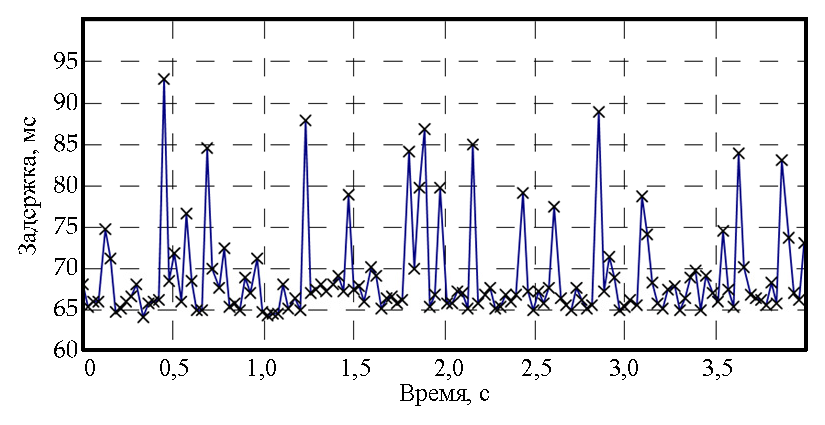
\includegraphics{localCongest.eps}
  \caption{Пример перегрузки в локальной сети \cite{clark}}
  \label{img:localCongest}
\end{figure}

\subsection{Перегрузки в канале доступа (тип 3) } \label{subsect2_1_3}
Доступ к каналу доступа, как правило, является одним из основных источников джиттера, поскольку он представляют собой одно из узких мест на пути пакета (рис. \ref{img:accessCongest}). Например, задержка сериализации IP-пакета в 1500 байт, посланного через T1 (1.544Mbit), будет около 8 миллисекунд, поэтому если в очереди перед речевой пакетом находятся пять пакетов данных, то вводится дополнительная задержка в 40 мс. Эта проблема может быть очень серьезной в случае ISDN, ADSL или в случае кабельных модемов, у которых пропускная способность исходящего канала дополнительно ограничена, например, если пропускная способность исходящего канала составляет 384кбит/в секунду, то каждый 1500 байтовый IP пакет в очереди введет дополнительную задержку в 30 мс.

\begin{figure} [h]
  \center
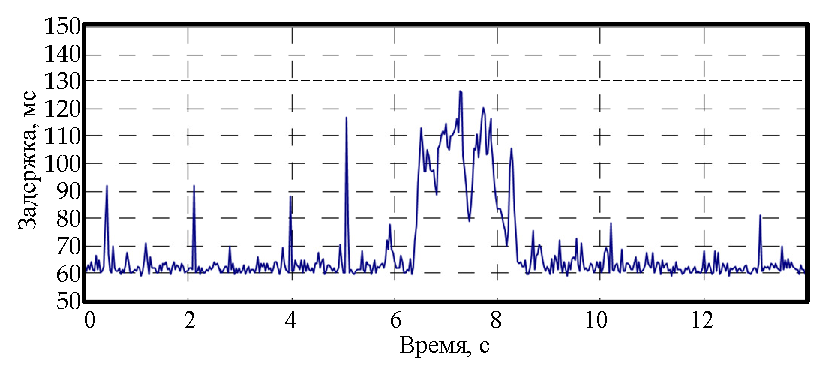
\includegraphics{accessCongest.eps}
  \caption{Пример перегрузки сети доступа \cite{clark}}
  \label{img:accessCongest}
\end{figure}

\subsection{Распределение нагрузки между несколькими линиями доступа или сервис провайдерами (тип 2) } \label{subsect2_1_4}
В целях предоставления предприятию VoIP доступа, предприятие может быть подключено через несколько сетей доступа к одному сервис провайдеру или направлять VoIP трафик через несколько независимых провайдеров. Это может привести к джиттеру если задержки на каждом канале доступа существенно различается.

\subsection{Распределение нагрузки (тип 2) } \label{subsect2_1_5}
Некоторые сервис провайдеры распределяют трафик через несколько внутренних маршрутов в пределах их сетей в целях повышения устойчивости и обеспечения более равномерной загрузки на сеть. Это вносит джиттер в результате разницы в задержке на каждом маршруте.

\subsection{Внутреннее разделение нагрузки в маршрутизаторах (тип 2) } \label{subsect2_1_6}
Для того чтобы поддерживать высокую скорость обработки некоторые маршрутизаторы используют многопроцессорные подход, при котором пакеты обрабатываются в нескольких параллельных очередях. Это может привести к небольшому уровню джиттера из-за различия в размере очереди.

\subsection{Высоко приоритетный служебный трафик (тип 1) } \label{subsect2_1_7}
Маршрутизаторы периодически генерируют трафик обновления с высоким приоритетом (рис. \ref{img:routeTraffic}) и выполняют обновления таблицы маршрутизации. Каждое такое событие может привести к задержке небольшого количества пакетов. Кроме того во время обновления таблицы маршрутизации могут существовать кратковременные петли, что может привести к чрезвычайно высокой задержке для отдельных пакетов (рис. \ref{img:routeChange}).

\begin{figure} [h]
  \center
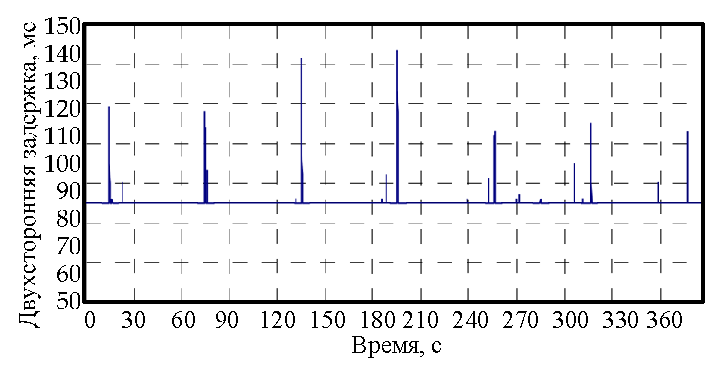
\includegraphics{routeTraffic.eps}
  \caption{Периодическое обновление таблицы маршрутизации без изменения маршрута \cite{clark}}
  \label{img:routeTraffic}
\end{figure}
\begin{figure} [h]
  \center
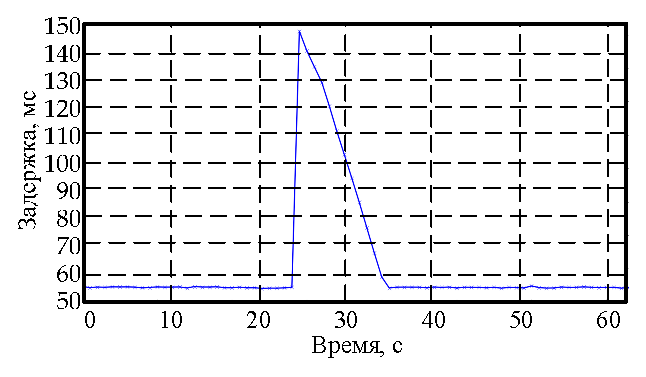
\includegraphics{routeChange.eps}
  \caption{Периодическое обновление таблицы маршрутизации при изменении маршрута \cite{clark}}
  \label{img:routeChange}
\end{figure}

\section{Анализ основных причин джиттера в беспроводной сети LTE} \label{sect2_2}
Беспроводная сеть налагает дополнительные факторы ухудшающие качество передачи. Далее рассмотрим влияние различных факторов на качество обслуживания, для услуг реального времени поверх сети LTE. Для моделирования и анализа ухудшающих факторов воспользуемся сетевым симмулятором NS3.

\subsection{Хэндовер}  \label{sect2_2_1}
Хэндовер (англ. Handover), является процессом передачи сессии абонента от одной базовой станции к другой. Может быть несколько причин для проведения передачи сессии:
\begin{itemize}
\item Когда абонент уходит с зоны покрытия одной ячейкой сети и входит в зону покрытия другой ячейкой. Хэндовер позволяет абонентам не быть привязанным к какой-либо географической точке и дает возможность передвигаться в пределах сети оператора без разрыва соединения.
\item Когда ёмкость сети в текущей ячейке израсходована при существовании соединения, которое находится в зоне, перекрытой другой ячейкой, передаётся к этой ячейке в порядке освобождения ёмкости первой ячейки для других ее пользователей, которые могут быть соединены только с первой ячейкой.
\item Когда канал используемый абонентом сильно зашумлён помехами, соединение передаётся другому каналу в той же ячейке или другому каналу в другой ячейке для устранения помех.
\item Когда абонент входит в зону микроячейки, соединение может быть передано для освобождения емкости большой сети.
\end{itemize}
Проведем моделирование влияния хэндовера на сквозную задержку в сети LTE в сетевом симмуляторе NS3. Детали стенда для моделирования описаны в Приложение \ref{AppendixA}. На рис. \ref{img:hand} избражено изменение сквозной сетевой задержки прибытия пакетов из-за 3-х переключений сессии абонента между базовыми станциями выполненными через некоторый промежуток времени. Также стоит заметить что при первой установке соединения задержка прибытия пакетов тоже была не стационарна.

\begin{figure} [h]
  \center
\includegraphics{hand.eps}
  \caption{Изменение задержки прибытия пакетов при хэндовере между базовыми станциями}
  \label{img:hand}
\end{figure}

\subsection{Расстояния между абонентом и базовой станцией}  \label{sect2_2_2}
Проведем моделирование влияния расстояния между абонентом и базовой станцией на скорсть передачи в канале сети LTE в сетевом симмуляторе NS3. Детали стенда для моделирования описаны в Приложение \ref{AppendixB}. В моделировании воспользуемся моделью потерь сигнала при распространнени Фрииса, которая впервые была описана в \cite{Friis}. Данная модель описывается следующей простой формулой передачи для радиоканала состоящего из передающей и приемной антены в свободном пространстве:

\begin{equation}\label{eq:friisMod1}
\frac{P_{r}}{P_{t}}=\frac{A_{r}A_{t}}{d^{2}\lambda^{2}},
\end{equation}

\noindent где для случая с изотропной антеной, без тепловых потерь $A_{isotr.}=\frac{\lambda^{2}}{4\pi}$ получим следующие уравнение:

\begin{equation}\label{eq:friisMod2}
\frac{P_{r}}{P_{t}}=\frac{\lambda^{2}}{(4\pi d)^{2}},
\end{equation}

\noindent cовременным представлением этого уравнения является:

\begin{equation}\label{eq:friisNew}
P_{r}=\frac{P_{t}G_{t}G_{r}\lambda^{2}}{(4\pi d)^{2}L},
\end{equation}

\noindent где $P_{r}$ - мощность полученного сигнала (Вт), $P_{t}$ - мощность отправленного сигнала (Вт), $G_{t}$ - коэффициент передачи, $G_{r}$ - коэффициент приема, $\lambda$ - длина волны (м), $d$ - расстояние (м), $L$ - системные потери. Как ожидалось (рис. \ref{img:Sinr_dist}) с увеличением расстояния между абонентом и базовой станцией уменьшается отношение сигнал шум с внутриситемными помехами включительно (SINR).

Для того чтобы рассчитать влияние SINR на скорость в канала рассмотрим формирование кадров в LTE (рис. \ref{img:frame_lte}). Рассмотрим нисходящее направление соединения и предположим что соединение между UE и eNB уже было установленно. Данные сначала поступают на PDCP (Packet data compression protocol) уровень. Этот уровень выполняет сжатие и шифрование данных и если необходимо устанавливает проверку на целосность. Далее данные передаются на RLC (LTE Radio Link Control) уровень, который объединяет PDCP PDUs в один RLC PDU.

RLC уровень объединит или сегментирует данные, поступающие от уровня PDCP в правильный размер блока и направит его на уровень МАС со своим собственным заголовком. Теперь MAC уровень выбирает схему модуляции и кодирования настраиваемую на физическом уровне. Теперь эти данные включенные в транспортный блок, должны быть переданы в 1 мс подкадре.

Теперь, сколько битов передаются в этом 1 мс размер транспортного блока? Это зависит от MCS (схемы модуляции и кодирования) и количество ресурсных блоков назначены UE. Мы должны обратиться к таблице 7.1.7.1-1 и таблице 7.1.7.2.1-1 от \cite{3GPPTS36213}.

(рис. \ref{img:mcs_dist})

(рис. \ref{img:tb_dist})

(рис. \ref{img:speed_dist})
\begin{figure} [H]
  \center
\includegraphics{Sinr_dist.eps}
  \caption{Зависимость нисходяшего канала передачи SINR от растояния между абонентом и базовой станцией}
  \label{img:Sinr_dist}
\end{figure}

\begin{figure} [h]
  \center
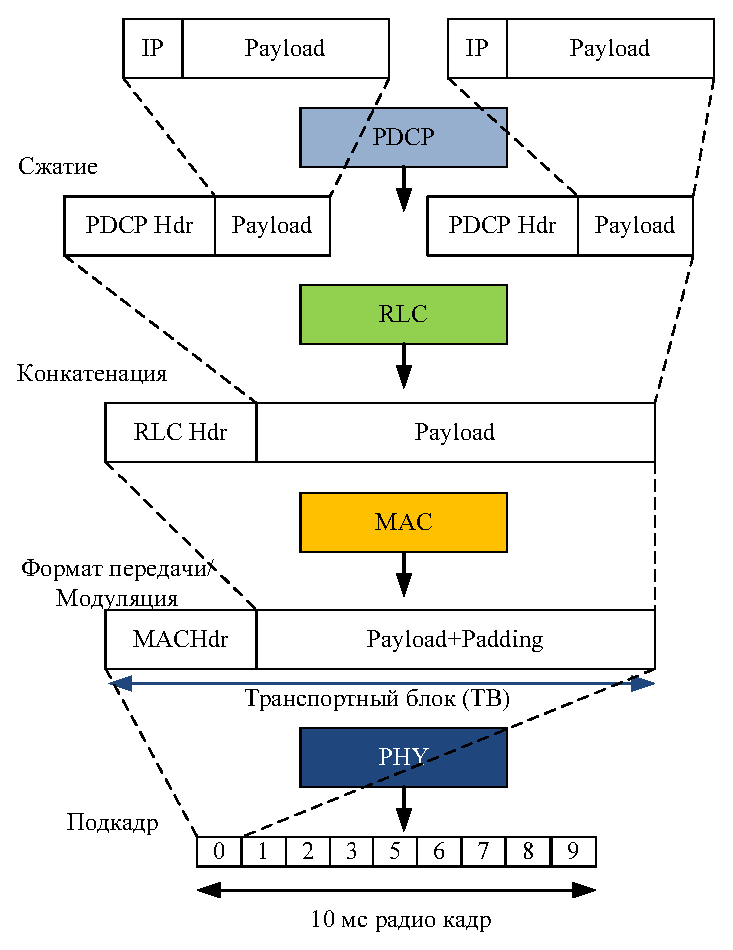
\includegraphics{frame_lte.eps}
  \caption{Формироваие транспортного блока (TB) в LTE}
  \label{img:frame_lte}
\end{figure}

\begin{figure} [h]
  \center
\includegraphics{mcs_dist.eps}
  \caption{Зависимость MCS нисходяшего канала передачи от растояния между абонентом и базовой станцией}
  \label{img:mcs_dist}
\end{figure}

\begin{figure} [h]
  \center
\includegraphics{tb_dist.eps}
  \caption{Зависимость размера TB нисходяшего канала передачи от растояния между абонентом и базовой станцией}
  \label{img:tb_dist}
\end{figure}

\begin{figure} [h]
  \center
\includegraphics{speed_dist.eps}
  \caption{Зависимость скорости нисходяшего канала передачи от растояния между абонентом и базовой станцией}
  \label{img:speed_dist}
\end{figure}


\subsection{Внутрисистемные помехи}  \label{sect2_2_3}
В этом документе рассматривается влияние всплесков внутрисистемных помех на качество обслуживания, особенно для услуг в реальном времени по верх сети LTE. Всплеск внутрисистемных помех может быть вызван другой базовой станцией, которая работает в том же диапазоне, хотя воздействие не зависит от источника помех.
Анализ описывает, как всплески помех влияет на характеристики канала в том числе на джиттер и  потери пакетов. Анализ затем использует поведение буфера дрожания для определения влияния на звонки VoIP. ITU-T E-модель используется для определения влияния на удовлетворенность пользователей.

LTE сети, внутрисистемные помехи и характеристики канала
Сотовые сети использовать канал кодирования и используют перемежение для борьбы с всплесками внутрисистемных помех. Тем не менее, блоковые ошибки возникают, когда условия канала достаточно плохи. Это приводит к потери пакетов для IP услуг, таких как FTP и VoIP. LTE использует повторные передачи чтобы поддерживать определенный уровень потери пакетов, что является достаточно низким, что не является достаточным чтобы предоставить хорошее качество для соответствующей услуги. Результат применения повторной передачи является то, что задержка пакета будет варьироваться, так называемый джиттер задержки.
В LTE передачи часто запланирована так чтобы синхронизироваться с замираниями, таким образом, что пакеты передавались к и от пользователей, имеющих наилучшие канальные условия, а пользователей, которые испытывают провалы замирания должны ждать, пока условия канала не будут улучшены. Это означает, что пакеты в очереди передачи будут испытывать различные задержки из-за планирования.
LTE также ограничивает количество повторных передач, чтобы избежать использования слишком большого количества ресурсов передачи для пользователей, которые испытывают деградацию характеристик канала. Это означает, что потери пакетов могут происходить в дополнение джиттеру задержки. Для услуг в реального времени, характерно чтобы пакеты могли быть повторно переданы со сквозной задержкой передачи до 50-100 мс.
Концептуальный пример задержки пакетов, которые могут произойти в присутствии внутрисистемных помех, показан на рис 1.

\begin{figure} [h]
  \center
\includegraphics{Sinr_inter.eps}
  \caption{Зависимость нисходяшего канала передачи SINR от растояния между абонентом и базовой станцией}
  \label{img:Sinr_inter}
\end{figure}

\begin{figure} [h]
  \center
\includegraphics{mcs_inter.eps}
  \caption{Зависимость MCS нисходяшего канала передачи от растояния между абонентом и базовой станцией}
  \label{img:mcs_inter}
\end{figure}

\begin{figure} [h]
  \center
\includegraphics{tb_inter.eps}
  \caption{Зависимость размера TB нисходяшего канала передачи от растояния между абонентом и базовой станцией}
  \label{img:tb_inter}
\end{figure}

\begin{figure} [h]
  \center
\includegraphics{speed_inter.eps}
  \caption{Зависимость скорости нисходяшего канала передачи от растояния между абонентом и базовой станцией}
  \label{img:speed_inter}
\end{figure}


\clearpage




